\documentclass[11pt,a4paper]{report}

% PACKAGES
\usepackage[ansinew]{inputenc}
\usepackage[T1]{fontenc}

\usepackage{graphicx}
\usepackage[usenames,dvipsnames]{xcolor}
\usepackage{listings}
\usepackage{multicol}
\usepackage{color}
\usepackage[ngerman,english]{babel}
\usepackage[hmargin=25mm,top=25mm]{geometry}
\usepackage{caption}
\usepackage{subcaption}
\usepackage{lmodern}
\usepackage{indentfirst}	% "tab" begin paragraph
\usepackage{hyperref} 
\usepackage{amsmath}
\usepackage{amssymb}
\usepackage{epstopdf}
\usepackage{multirow}
\usepackage{color, colortbl}
\usepackage{todonotes}

%\renewcommand{\labelenumi}{\arabic{enumi}.}
%\renewcommand{\labelenumii}{\arabic{enumi}.\arabic{enumii}}

\hypersetup{
  colorlinks,
  citecolor=violet,
  linkcolor=Peach,
  urlcolor=green}

\thispagestyle{empty}
\lstset{
	basicstyle=\footnotesize\ttfamily,
	numberstyle=\tiny,         
  numbersep=5pt,             
  tabsize=2,                 
  extendedchars=true,         
  breaklines=true,            
  keywordstyle=\color{red},
	frame=b,         
  stringstyle=\color{white}\ttfamily, 
  showspaces=false,           
  showtabs=false,            
  xleftmargin=17pt,
  framexleftmargin=17pt,
  framexrightmargin=5pt,
  framexbottommargin=4pt,
  showstringspaces=false          
 }
% 
\lstloadlanguages{Java}
%  
\DeclareCaptionFont{white}{\color{white}}
\DeclareCaptionFormat{listing}{\colorbox[cmyk]{0.43, 0.35, 0.35,0.01}{\parbox{\textwidth}{\hspace{15pt}#1#2#3}}}
%\captionsetup[lstlisting]{format=listing,labelfont=white,textfont=white, singlelinecheck=false, margin=0pt, font={bf,footnotesize}}

\begin{document}
\selectlanguage{english}

% TITLEPAGE
%=============================================================================================
\begin{figure}[t]
	
\includegraphics[height=12.9mm]{graphics/logos/laas.jpeg}
	\hfill
	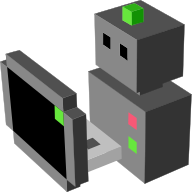
\includegraphics[height=20.9mm]{graphics/logos/morse.png}
\end{figure}

\vspace*{3\baselineskip}

\begin{center}
	
	\huge{\textbf{List of possible bugs detected in Morse Simulator}}\\[3\baselineskip]
	
\end{center}

\begin{raggedleft}
	{\Large
		\textbf{Simulation and communications management in a multi-robot environment}\\
		\emph{Internship}\\[2\baselineskip]
		
		Paulo Lopes Sim�es\\[2\baselineskip]
		
		\textbf{Supervisor(s)}\\
		Simon Lacroix\\
		
		
		\vfill
		
		LAAS-CNRS\\
		Toulouse, France\\
	}
	
\end{raggedleft}

\begin{raggedright}
	
	{\large
		\vfill
		\begin{tabbing}
			
			\hspace*{4cm} \= \kill
			Begin date of exercise: \> 01.10.2013\\
			Filing date: \> 31.12.2013\\
			
		\end{tabbing}
	}
	
\end{raggedright}
\newpage

\setcounter{page}{1}
\pagenumbering{roman}

%\tableofcontents
%\newpage

% MAIN MATTER
%=============================================================================================
\setcounter{page}{1}
\pagenumbering{arabic}

\chapter*{List of possible bugs detected}

\begin{enumerate}
\item The robot \textbf{Jido()} doesn't fall with gravity:

\textit{jido.translate(x=-5, z=1)}.... It is levitating all the time with this 'z' coordinate.

\item Documentation of \textbf{Supervision Services} doesn't present all methods like \textit{$get\_all\_stream\_ports$}.
\url{http://www.openrobots.org/morse/doc/latest/user/supervision_services.html}

\item Class \textbf{Quadrotor()}, 2 different robots with the same name? The 2nd is the default (?)

\url{http://www.openrobots.org/morse/doc/latest/user/robots/quadrotor.html}

\url{http://www.openrobots.org/morse/doc/latest/user/robots/quadrotor_dynamic.html}

\item Error related with \textbf{Waypoint()} usage -> Radar (Left or Right). For example, running the script bellow, the B21 robot tries to stay in its initial position. Using the ATRV, if we constantly push B21 away from this initial (or other destination) point, at some moment the Blender quits and enunciates the errors shown in XXX.

Script: \url{https://raw.github.com/pauloet/morse/master/My_Simulations/bug1.py}



\end{enumerate}



\end{document}
